\documentclass[german, master, utf8, pdftex, dvipsnames]{base/thesis_KBS}

\usepackage{units}    % \unit[23]{m}
\usepackage{nicefrac} % \nicefrac{km}{h}
\usepackage{environ}
\usepackage[justification=centering]{subcaption} % mehrere Bilder in einer figure
\usepackage{pgfplots} % Plots für Benchmarks
\usepackage{csquotes} % Anführungszeichen
\usepackage{float} % figure platzieren
\usepackage{listings} % Code einfügen
\usepackage{tabto} % Einrückung zu einer festen Position
\usepackage{pdfpages} % Einfügen der Erklärung am Ende
\usepackage[shortlabels]{enumitem} % Mehr Optionen für enumerate
\usepackage{xfrac} % Bessere Brüche
\usepackage{booktabs} % Bessere Tabellen
\usepackage[protrusion=false,spacing=true]{microtype} % Bessere Text Skalierung
\usepackage{subfiles} % include
\usepackage{silence} % Unterdrückung von Warnungen
\usepackage[figuresright]{rotating} % Bilder rotieren
\usepackage{amsmath}
\usepackage{makecell}
\usepackage{mathtools}
\newcommand*\colvec[1]{\begin{pmatrix}#1\end{pmatrix}}

\usepackage{xargs}                      % Use more than one optional parameter in a new commands
%\usepackage[pdftex, dvipsnames]{xcolor}  % Coloured text etc.
\usepackage{xcolor}
% 
\usepackage[colorinlistoftodos,prependcaption,textsize=tiny]{todonotes}
\newcommandx{\unsure}[2][1=]{\todo[linecolor=orange,backgroundcolor=orange!25,bordercolor=orange,#1]{#2}}
\newcommandx{\change}[2][1=]{\todo[linecolor=blue,backgroundcolor=blue!25,bordercolor=blue,#1]{#2}}
\newcommandx{\info}[2][1=]{\todo[linecolor=green,backgroundcolor=green!25,bordercolor=green,#1]{#2}}
\newcommandx{\improvement}[2][1=]{\todo[linecolor=red,backgroundcolor=red!25,bordercolor=red,#1]{#2}}
\newcommandx{\thiswillnotshow}[2][1=]{\todo[disable,#1]{#2}}

\usepackage{algorithm, algorithmicx, algpseudocode}  % for pseudo code (cf. documentation)
\renewcommand{\algorithmiccomment}[1]{\qquad{\small // \textit{#1}}}
\newcommand{\INDSTATE}[1][1]{\hspace{#1\algorithmicindent}}
\let\OldStatex\Statex
\renewcommand{\Statex}[1][3]{%  for pseudo code indentation
  \setlength\@tempdima{\algorithmicindent}%
  \OldStatex\hskip\dimexpr#1\@tempdima\relax}

\pgfplotsset{compat=1.16} % pgfplots config
\setquotestyle{american} % csquotes config
\raggedbottom % verhindert Lücken zwischen Überschriften und Text
\hyphenpenalty=750 % macht Worttrennung seltener

\NewEnviron{myequation}{	
	\begin{equation}
		\scalebox{1.2}{$\BODY$}
	\end{equation}
}

\DeclarePairedDelimiter\abs{\lvert}{\rvert}%
\DeclarePairedDelimiter\norm{\lVert}{\rVert}%

% Swap the definition of \abs* and \norm*, so that \abs
% and \norm resizes the size of the brackets, and the 
% starred version does not.
\makeatletter
\let\oldabs\abs
\def\abs{\@ifstar{\oldabs}{\oldabs*}}
%
\let\oldnorm\norm
\def\norm{\@ifstar{\oldnorm}{\oldnorm*}}
\makeatother
	

\WarningFilter*{microtype}{I cannot find}

% verhindert (meistens) Zeilenumbrüche vor Verweisen
%\NewCommandCopy{\oldref}{\ref}
%\renewcommand{\ref}[1]{\nolinebreak \oldref{#1}}
%\NewCommandCopy{\oldcite}{\cite}
%\renewcommand{\cite}[1]{\nolinebreak \oldcite{#1}}

\newcommand{\pleasedontaddwhorechildren}{\newpage}

\lstset{
    basicstyle=\ttfamily\small,
    numberstyle=\footnotesize,
    numbers=left,
    backgroundcolor=\color{gray!10},
    frame=single,
    tabsize=2,
    rulecolor=\color{black!30},
    title=\lstname,
    escapeinside={\%*}{*)},
    breaklines=true,
    breakatwhitespace=true,
    framextopmargin=2pt,
    framexbottommargin=2pt,
    showstringspaces=false
    inputencoding=utf8,
    extendedchars=true,
    literate={ä}{{\"a}}1 {ö}{{\"o}}1 {ü}{{\"u}}1 {ß}{{\ss}}1 {∆}{{$\Delta$}}1,
}

%%%%%%%%%%%%%%%%%%%%%%%%%%%%%%%%%%%%%%%%%%%%%%%%%%%%%%%%%%%%%%%%%%%%%%%%%%%%%%%

\begin{document}

\title{Loop Closure in TSDF basiertem SLAM} % Deckblatt
\shorttitle{Loop Closure in TSDF basiertem SLAM} % Für Titel am unteren Rand der Seiten

\author{Patrick Hoffmann}
\email{pahoffmann@uni-osnabrueck.de}
\firstSupervisor{Prof. Dr. Mario Porrmann}
\secondSupervisor{Alexander Mock, M. Sc.}
% \submitdate{August 2022}             % by default current month & year
%signline{Osnabrück, 11. Dezember 2004} % by default "signcity, submitdate"

\generatetitle

\cleardoublepage

\begin{prefacesection}{Zusammenfassung}

Die vorliegenden Arbeit liefert eine Lösung zum Schleifenschluss-Problem in einem \emph{Truncated Signed Distance Field (TSDF)} basiertem \emph{Simultaneaous Localization and Mapping (SLAM)} Ansatz. Beschrieben ist die Konzeption und Algorithmik für eine Detektion von Schleifenschlüssen und die anschließende, mehrschrittige Validierung über im Rahmen der Arbeit entwickelte Validatoren, die fehlerhafte Schleifenschlüsse aussortierten und so für eine robustere Optimierung des Pose-Graphen sorgen. Darüber hinaus sind mehrere in der Arbeit entwickelte Strategien zum Update der volumetrischen TSDF-Kartenrepräsentation dargelegt. Dabei handelt es sich um ein globales Update der Karte und zwei darauf basierte, partielle Kartenupdates, die eine deutliche laufzeittechnische Optimierung gegenüber dem globalen Update ermöglichen.

\end{prefacesection}

\vspace{5cm}

\begin{prefacesection}{Abstract}

The present thesis provides a solution to the loop closure problem in a \emph{Truncated Signed Distance Field (TSDF)} based \emph{Simultaneaous Localization and Mapping (SLAM)} approach. Described is the design and algorithm for a loop closure detection and subsequent multi-step validation via validators developed as part of the thesis, which sorted out erroneous loop closures to provide more robust optimization of the pose graph. In addition, several strategies developed in the work are outlined for updating the volumetric TSDF map representation. These are a global update of the map and two partial map updates based upon it, which provide significant runtime optimization over the global update.

\end{prefacesection}


\cleardoublepage
\tableofcontents


\startTextChapters %%%%%%%%%%%%%%%%%%%%%%%%%%%%%%

% Einleitung + Motivation
\subfile{chapters/einleitung}

% Stand der Technik
\subfile{chapters/standdertechnik}

% verwendete libraries
%\subfile{chapters/libraries}

% tsdf, slam, loop closure
\subfile{chapters/grundlagen}

\subfile{chapters/daten_assoziationen}

\subfile{chapters/loopclosure}

\subfile{chapters/map_update}

\subfile{chapters/ausblick}

\appendix

\subfile{chapters/appendix}


\bibliography{papers.bib}                                                                                                                           

\cleardoublepage

\improvement{Endpage für Unterschrift einbauen}
%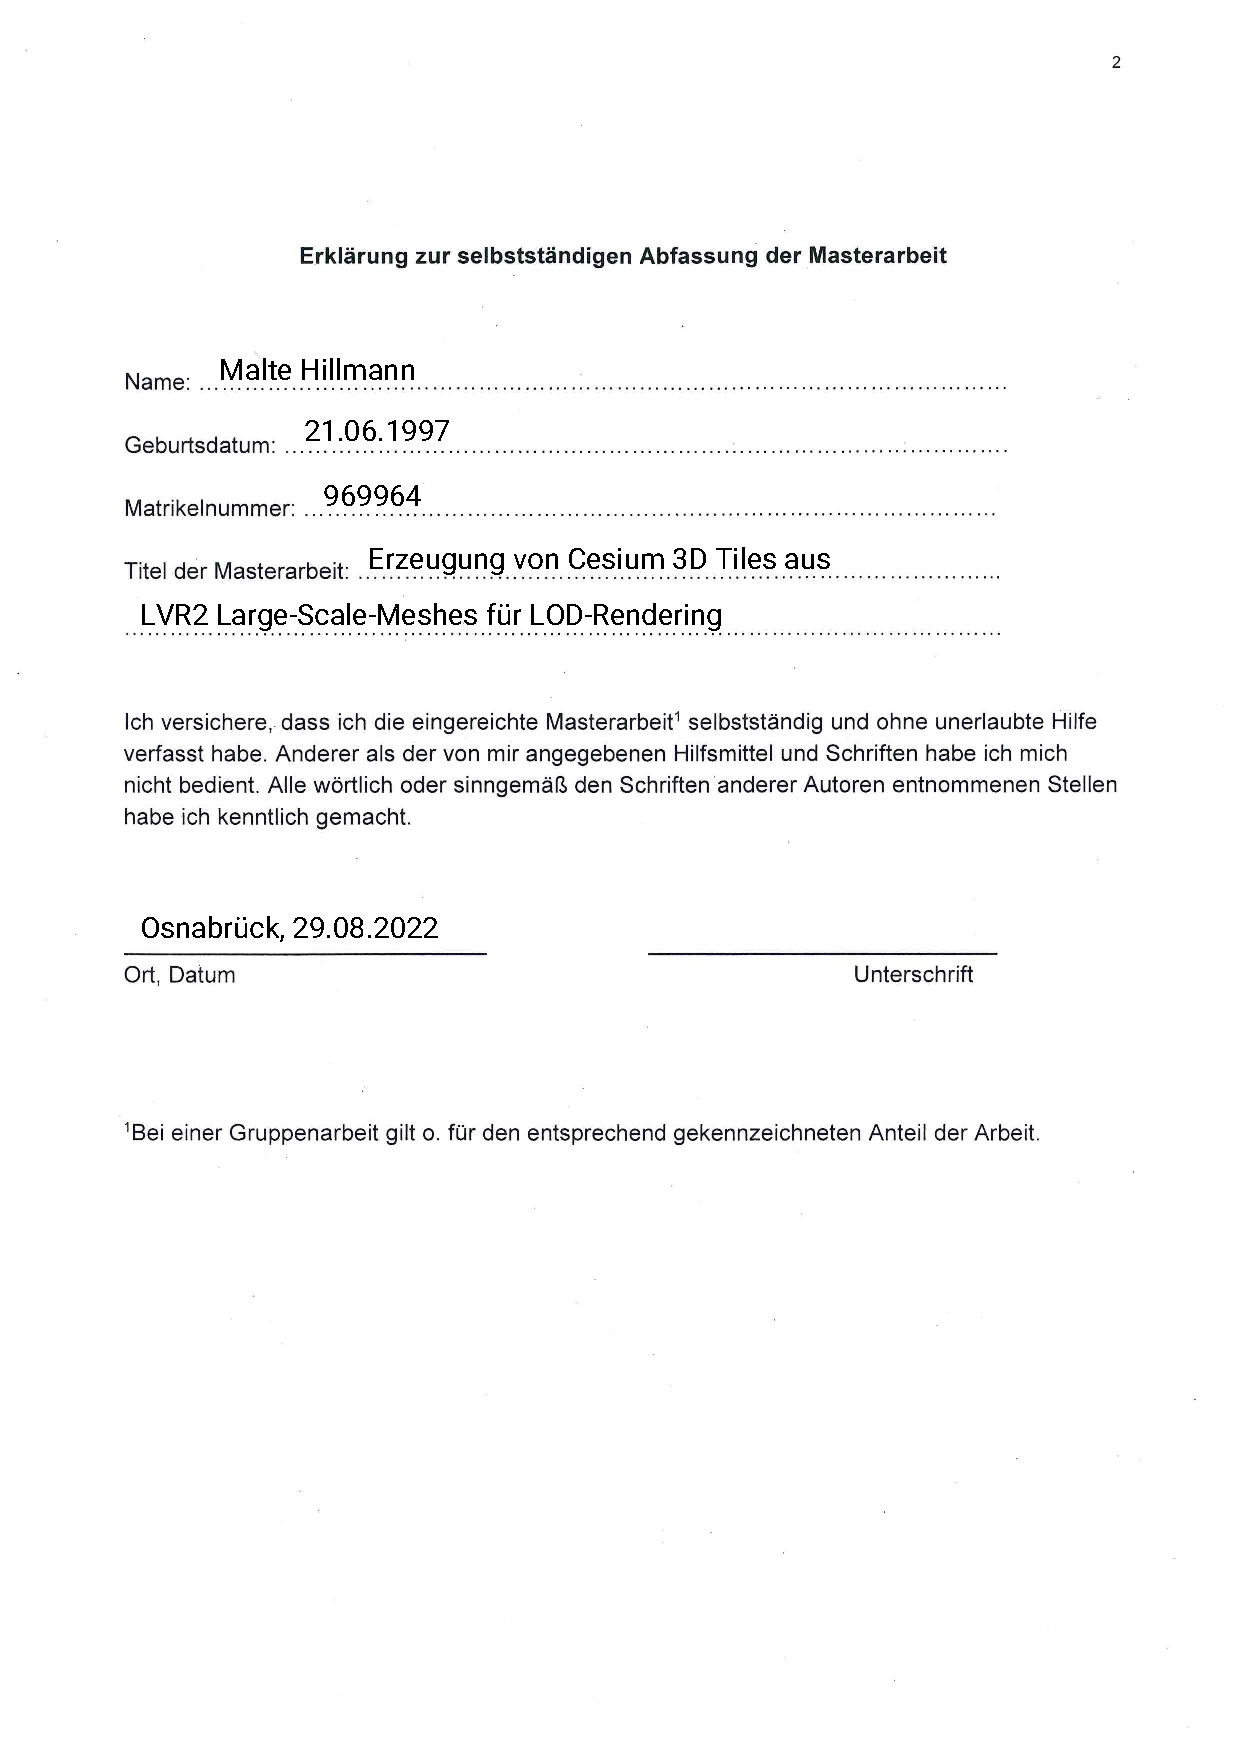
\includepdf[pages=-]{pics/endpage.pdf} %%%%%%%%%%%%%%%%%%%%%%%%%%%%%%

\end{document}
